\documentclass[10pt,letterpaper]{article}
\usepackage[margin=0.78in,headheight=17pt]{geometry}
\usepackage[T1]{fontenc}
\usepackage[utf8]{inputenc}
\usepackage{lmodern,microtype,parskip}
\usepackage{amsmath,amssymb}
\usepackage{xcolor,booktabs,longtable,tabularx,array,enumitem}
\usepackage[most]{tcolorbox}
\usepackage{fancyhdr,lastpage,titlesec,hyperref,listings}
\usepackage{tikz}
\usetikzlibrary{arrows.meta,positioning,shapes.geometric}
\definecolor{navy}{HTML}{17324D}
\definecolor{bluegray}{HTML}{43657D}
\definecolor{lightblue}{HTML}{EAF2F8}
\definecolor{linegray}{HTML}{CBD5DF}
\definecolor{softgray}{HTML}{F3F5F7}
\definecolor{accent}{HTML}{8E3B46}
\hypersetup{colorlinks=true,linkcolor=navy,urlcolor=bluegray,pdfborder={0 0 0}}
\urlstyle{same}
\titleformat{\section}{\Large\bfseries\color{navy}}{\thesection}{0.6em}{}
\titleformat{\subsection}{\large\bfseries\color{bluegray}}{\thesubsection}{0.5em}{}
\setlist[itemize]{leftmargin=*,itemsep=3pt,topsep=3pt}
\setlist[enumerate]{leftmargin=*,itemsep=3pt,topsep=3pt}
\setlength{\emergencystretch}{3em}
\renewcommand{\arraystretch}{1.22}
\setlength{\tabcolsep}{4pt}
\pagestyle{fancy}\fancyhf{}
\lhead{Secure Programming \& SAST Engineering}
\rhead{Engineering Documentation Suite}
\cfoot{\thepage\ / \pageref{LastPage}}
\newcolumntype{Y}{>{\raggedright\arraybackslash}X}
\newcommand{\checkbox}{\(\square\)}
\newcommand{\blankline}{\noindent\rule{\linewidth}{0.35pt}\par\vspace{4pt}}
\newcommand{\writearea}[1]{\par\begin{tcolorbox}[colback=white,colframe=linegray,boxrule=0.5pt,height=#1,sharp corners]\mbox{}\end{tcolorbox}\par}
\newtcolorbox{focusbox}[1]{colback=lightblue,colframe=bluegray,title=\textbf{#1},fonttitle=\bfseries,breakable}
\newtcolorbox{warnbox}[1]{colback=softgray,colframe=accent,title=\textbf{#1},fonttitle=\bfseries,breakable}
\lstset{basicstyle=\ttfamily\footnotesize,breaklines=true,frame=single,rulecolor=\color{linegray},backgroundcolor=\color{softgray},showstringspaces=false,columns=fullflexible,keepspaces=true,upquote=true}

\begin{document}
\begin{titlepage}
\vspace*{1.0in}
{\color{bluegray}\Large Curriculum}\\[1.0em]
{\color{navy}\Huge\bfseries Prerequisite-Based SAST Curriculum}\\[0.7em]
{\Large Twelve-week chapter crosswalk, competency gates and capstone}\\[2.0em]
\rule{\linewidth}{1.0pt}
\vfill
\textbf{Source discipline:} Book-derived foundations are identified separately from current engineering extensions.\\
\textbf{Edition:} 29 October 2026
\end{titlepage}
\tableofcontents
\clearpage
\begin{focusbox}{Learning contract}
Prerequisites are directed edges: complete the prerequisite modules and practical gate before starting dependent activities. A week number is a planning estimate, not a substitute for demonstrable competency. Assignments use synthetic or expressly authorized code only.
\end{focusbox}
\section{Prerequisite DAG}
\begin{center}
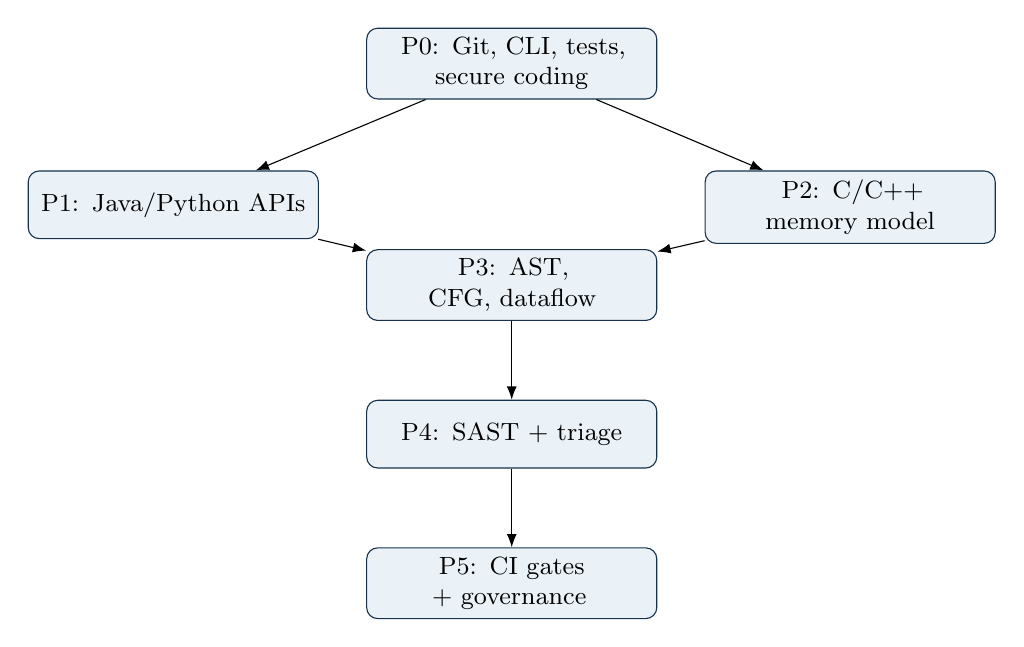
\begin{tikzpicture}[>=Latex,node distance=10mm,box/.style={draw=navy,fill=lightblue,rounded corners,text width=3.45cm,align=center,minimum height=0.86cm,font=\small}]
\node[box](a){P0: Git, CLI, tests, secure coding};\node[box,below left=9mm and 6mm of a](b){P1: Java/Python APIs};\node[box,below right=9mm and 6mm of a](c){P2: C/C++ memory model};
\node[box,below=19mm of a](d){P3: AST, CFG, dataflow};\node[box,below=of d](e){P4: SAST + triage};\node[box,below=of e](f){P5: CI gates + governance};
\draw[->](a)--(b);\draw[->](a)--(c);\draw[->](b)--(d);\draw[->](c)--(d);\draw[->](d)--(e);\draw[->](e)--(f);
\end{tikzpicture}
\end{center}
\section{Entry prerequisites and diagnostic}
\begin{enumerate}
\item \textbf{Foundational programming}: functions, error handling, test frameworks, package/build management, version control, and CLI tool hygiene.
\item \textbf{Security foundations}: CIA impact, trust boundaries, injection, authorization, privacy/secret classifications and responsible research.
\item \textbf{Language literacy}: Java exceptions and JDBC; C pointer, array and size types; Python file/path/process APIs.
\item \textbf{Program analysis literacy}: AST versus source text, dataflow joins, call graphs and sanitization contracts.
\end{enumerate}
Entry diagnostic: review 12 short snippets across three languages, map five CWEs, run one reproducible test harness and explain one CFG. An incomplete item becomes an individual remedial prerequisite rather than being waived by tenure.
\section{Teaching sequence and evidence gates}
\small
\begin{longtable}{@{}p{0.08\linewidth}p{0.25\linewidth}p{0.36\linewidth}p{0.23\linewidth}@{}}\toprule
Week & Textbook & Practical activity & Exit evidence\\\midrule\endhead
1 & Ch. 1, 2 & Threat properties and scanner taxonomy & Trust boundary sheet + calibration quiz\\
2 & Ch. 3 & Human triage cycle and metrics & Six finding dispositions\\
3 & Ch. 4 & AST/CFG and fixed-point taint & Annotated graph + trace\\
4 & Ch. 5 & Input, encoding and query safety & Parameter binding tests\\
5 & Ch. 6 & Buffer and string bounds & Reproducible C safety harness\\
6 & Ch. 7 & Checked integer arithmetic & Overflow edge-case tests\\
7 & Ch. 8 & Error and resource hygiene & Failure-path review\\
8 & Ch. 9 & Web and identity security & Route-level controls worksheet\\
9 & Ch. 10 & Structured parsers/services & XML external-entity review\\
10 & Ch. 11, 12 & Secrets and privilege & Least privilege threat model\\
11 & Ch. 13 & Java full-program review & Scan log + evidence package\\
12 & Ch. 14 & C/C++ review; capstone & Code scan + verified fixes + gate\\\bottomrule
\end{longtable}\normalsize
\section{Competency gates}
\subsection{G1: Conceptual foundations}
Score at least 80\% on reasoning-based chapter questions. Explain a false-positive example and a false-negative risk without relying on a vendor marketing claim.
\subsection{G2: Technical review}
Complete Java, C/C++ and Python laboratories; produce a trace for each; demonstrate secure behavior with both positive and rejection/edge tests. A screenshot alone is insufficient.
\subsection{G3: Analysis engineering}
Construct a CFG, define a monotone transfer function, implement or specify a custom rule with true-positive and false-positive fixtures, validate sample SARIF.
\subsection{G4: Operational readiness}
Produce a workflow threat model, deterministic scan plan, historical baseline, triage records, two closure records and a scored security gate. Unapproved suppressions fail this gate.
\section{Capstone specification}
An intentionally small, non-production polyglot sample contains three independently authored security-relevant anti-patterns. The participant must inventory scope, document threat assumptions, scan, triage, fix, test and rerun. The instructor plants a benign use case that triggers a broad pattern rule so students can demonstrate false-positive reasoning. \textbf{Submission:} commit identifiers, scan commands and tool versions; finding records and evidence; test results; sanitized SARIF; scorecards; and a concise residual-risk statement.
\section{Evaluation}
Technical correctness 30\%; evidence and reproduction 25\%; triage accuracy and impact reasoning 20\%; CI trust-boundary design 15\%; communication and traceability 10\%. Passing: 80\% overall, no major unauthorized testing or credential-handling defects, and all G1--G4 completed. Reattempts require new evidence rather than repackaged screenshots.
\section{Instructor operations}
Maintain a private answer key and separate seeded-defect manifests; version control instructions and fixtures; publish only synthetic credentials. Calibrate reviewers by blind-reviewing identical findings, discuss disagreements, then update rubric definitions. Do not benchmark teams by raw warning totals.
\end{document}
